\subsection{Γ 函数的性质}

命题 2. 对每个 x \textgreater{} 0 ，有

\[
\Gamma (x) = \lim _ {n \rightarrow \infty} \frac {n ^ {x} n !}{x (x + 1) \dots (x + n)}\tag{8}
\]

（高斯公式），以及

\[
\Gamma (x) = e ^ {- \gamma x} \frac {1}{x} \prod_ {n = 1} ^ {\infty} \frac {e ^ {x / n}}{1 + \frac {x}{n}}\tag{9}
\]

其中 \(\gamma\) 表示欧拉常数，且 (9) 右端的无穷乘积在 \(\mathbf{R}\) 的每个不含任何整数 \(< 0\) 的紧区间上绝对且一致收敛（魏尔斯特拉斯公式）。

函数 \(\Gamma(x)\) 在 \(]0, +\infty[\) 上无穷次可导，且有

\[
{\frac {\Gamma^ {\prime} (x)}{\Gamma (x)}} = - \gamma - {\frac {1}{x}} + \sum_ {n = 1} ^ {\infty} \left({\frac {1}{n}} - {\frac {1}{x + n}}\right)\tag{10}
\]

以及

\[
\mathrm{D} ^ {k} (\log \Gamma (x)) = \sum_ {n = 0} ^ {\infty} \frac {(- 1) ^ {k} (k - 1) !}{(x + n) ^ {k}} \quad \text { for } \quad k \geqslant 2,\tag{11}
\]

(10) 与 (11) 右端的级数在每个不含任何整数 \(\leqslant 0\) 的紧区间上绝对且一致收敛。

事实上，VII, p.~306 prop. 1 的证明表明

\[
\Gamma (x) = \lim _ {n \rightarrow \infty} \frac {n ^ {x} (n - 1) !}{x (x + 1) \dots (x + n - 1)}
\]

由此得高斯公式，因为 \(\frac{n}{x + n}\) 趋于 1 （当 \(n\) 趋于 \(+\infty\) 时）。还可以写

\[
\log \frac {n}{n - 1} = \frac {1}{n - 1} + \left(\log \frac {n}{n - 1} - \frac {1}{n - 1}\right),
\]

于是（用 prop. 1 的记号）

\[
\exp (u _ {n} (x)) = e ^ {x \left(\log \frac {n}{n - 1} - \frac {1}{n - 1}\right)} \frac {e ^ {x / n - 1}}{1 + \frac {x}{n - 1}}
\]

而以 \(\log \frac{n}{n - 1} -\frac{1}{n - 1}\) 为通项的级数绝对收敛且和为 \(-\gamma\) ，其中 \(\gamma\) 表示欧拉常数（V,p.242），由此得到魏尔斯特拉斯公式。

对 \(|x| \leqslant a\) ，有 \(\left|1/(x+n)^{k}\right| \leqslant 1/(n-a)^{k}\) （只要 n \textgreater{} a），故公式 (11) 右端的级数在 R 的每个不含任何整数 \(\leqslant 0\) 的紧区间上绝对且一致收敛（对任何整数 \(k \geqslant 2\) ）；同样的论证适用于 (10) 的右端，因为 \(\left|\frac{1}{n}-\frac{1}{x+n}\right| \leqslant \frac{a}{n(n-a)}\) （对 \(|x| \leqslant a\) 和 n \textgreater{} a）。由于这些级数是由级数

\[
\log \Gamma (x) = - \gamma x - \log x + \sum_ {n = 1} ^ {\infty} \left(\frac {x}{n} - \log \left(1 + \frac {x}{n}\right)\right)
\]

逐项求导得到的，而该级数对每个 \(x > 0\) 收敛，故以 \(\frac{x}{n} - \log \left(1 + \frac{x}{n}\right)\) 为通项的级数在含于 \([0, +\infty[\) 的每个紧区间上绝对且一致收敛，且对每个 x \textgreater{} 0 有 VII, p.~308 的关系式 (10) 与 (11) （II, p.~52, th. 1）。此外，对每个 \(x \in R\) ，只要 n 充分大，表达式 \(\frac{x}{n} - \log\left(1 + \frac{x}{n}\right)\) 就有定义，故 II, p.~52 的 th. 1 再次表明 (9) （VII, p.~307）右端的无穷乘积在每个不含任何整数 \(\leqslant 0\) 的紧区间上绝对且一致收敛。

函数 \(\Gamma(x)\) （对 x \textgreater{} 0 定义的）可以延拓到异于整数 \(\leqslant 0\) 的点 x 的全体所成之集上，使之在这个集上满足 VII, p.~307 的方程 (7) ：只需对 \(-(n + 1) < x < -n\) 置

\[
\Gamma (x) = \frac {1}{x (x + 1) \ldots (x + n)} \Gamma (x + n + 1).
\]

由 VII, p.~307 的 prop. 2 ，VII, p.~307 与 308 的公式 (8)、(9)、(10) 与 (11) （在 (11) 中以 \(\mathrm{D}^{k}(\log|\Gamma(x)|)\) 代替 \(\mathrm{D}^{k}(\log\Gamma(x))\)）在这个集上仍然成立。公式 (9) （VII, p.~307）表明当 x 趋于 0 时 \(\Gamma(x)\sim1/x\) ，于是由 VII, p.~307 的 (7) ，

\[
\Gamma (x) \sim \frac {(- 1) ^ {n}}{n ! (x + n)}
\]

当 \(x\) 趋于 \(-n\) （ \(n\) 为整数 \(\geqslant 0\) ）时成立。于是函数 \(1 / \Gamma(x)\) 可以用连续性延拓到整个 \(\mathbf{R}\) ，在整数 \(\leqslant 0\) 处赋以值 0 ；这样，对一切 \(x \in \mathbf{R}\)

\[
\frac {1}{\Gamma (x)} = \lim _ {n \rightarrow \infty} \frac {x (x + 1) \dots (x + n)}{n ^ {x} n !}\tag{12}
\]

以及

\[
\frac {1}{\Gamma (x)} = e ^ {\gamma x} x \prod_ {n = 1} ^ {\infty} \left(1 + \frac {x}{n}\right) e ^ {- x / n}\tag{13}
\]

并且可以如同 VII, p.~307 的 prop. 2 那样证明，(13) 右端的无穷乘积在 \(\mathbf{R}\) 的每个紧区间上绝对且一致收敛。

由于 \(\Gamma(x) > 0\) （对 \(x > 0\) ），VII, p.~307 的方程 (7) 表明：\(\Gamma(x) < 0\) （对 \(-(2n - 1) < x < -(2n - 2)\) ），而 \(\Gamma(x) > 0\) ，对

\[
- 2 n <   x <   - (2 n - 1)
\]

\((n \text{ 为整数 } \geqslant 1); \text{ 还 } \Gamma(x) \text{ 的右极限分别为 } +\infty \text{，在点 } -2n \text{；} -\infty \text{，在点 } -(2n+1), \text{ 且左极限分别为 } -\infty \text{，在点 } -2n \text{；} +\infty \text{，在点 } -(2n+1) \text{ (对所有 } n \in \mathbf{N}). \text{ VII 中的公式 (11)，p. 308 表明，对于 } k=2, \text{ 右端总是 } \geqslant 0 \text{（在其有定义时），因此}\)

\[
\Gamma^ {\prime \prime} (x) \Gamma (x) - \left(\Gamma^ {\prime} (x)\right) ^ {2} \geqslant 0,
\]

\pandocbounded{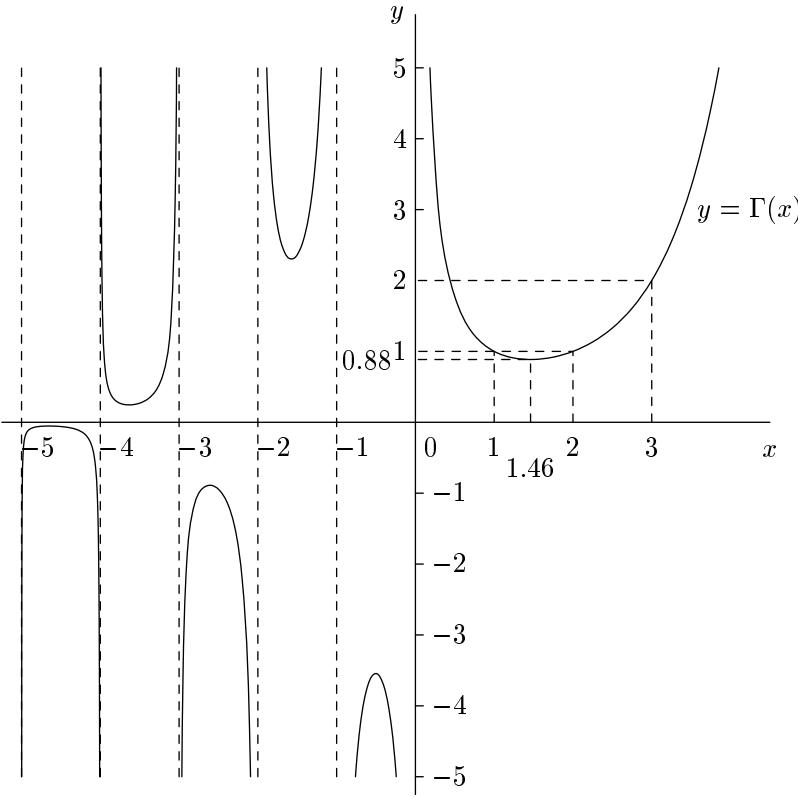
\includegraphics[keepaspectratio]{images/part002_cfbcc1f6.jpg}}\\
图 1\\
因而 \(\Gamma''(x)\) 与 \(\Gamma(x)\) 有相同的符号；于是 \(\Gamma\) 在 x \textgreater{} 0 时以及 \(-(2n + 2) < x < -(2n + 1)\) 时凸，在 \(-(2n + 1) < x - 2n\) 时凹（ \(n \in N\) ）；由此推出，在 \(\Gamma\) 凸的区间上，\(\Gamma'(x)\) 从 \(-\infty\) 递增到 \(+\infty\) ，而在 \(\Gamma\) 凹的区间上，\(\Gamma'(x)\) 从 \(+\infty\) 递减到 \(-\infty\) 。由此得到 \(\Gamma\) 的图像（图 1）。
% semantic-fragments: legacy-input-seam
\relax{}
